\section{保守力}\label{sec:06.04}

我们已经证明在引力作用下,质点的运动遵守下列形式的能
量守恒:
\begin{equation}\label{eqn:06.04.01}
    T + V =  \text{不变量}
\end{equation}
现在我们一般地来讨论在什么条件下上式成立或不成立,即满足
上式的运动应有什么性质。

我们曾指出,一般说来,作功是与路径有关的。因为从功的
定义$  A = T _ { 2 } - T _ { 1 }   $,一般并不能推出式 \eqref{eqn:06.04.01}。在引力情况,由于
有
\begin{equation}\label{eqn:06.04.02}
    A = V _ { 1 } - V _ { 2 }
\end{equation}
所以式\eqref{eqn:06.04.01}才成立。式\eqref{eqn:06.04.02}正是表示引力作功与路径无
关。

如果有摩擦力,情况就完全不同。我们来讨论图6.11的固定
斜面,设各面的摩擦系数均为$ \mu $。若质点沿$ 1 \to 2 $自由下落,则质点
只受重力作用,重力作功为
\begin{figurex}
    \centering
    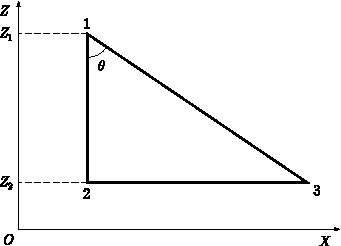
\includegraphics{figure/fig06.11}
    \caption{有摩擦力情况的作功}
    \label{fig:06.11}
\end{figurex}
% 180.jpg
\clearpage\mbox{}\vspace{-1em}
\begin{equation*}
    A _ { \text{重} _ { 1 \to 2 } } = m g \left| Z _ { 2 } - Z _ { 1 } \right|
\end{equation*}
而摩擦力作功为零,即
\begin{equation*}
   A _ { \text{摩} _ { 1 \to 2 } } = 0
\end{equation*}
质点沿$ 1 \to 3 $下滑,则位移大小为$ \dfrac { \left| Z _ { 2 } - Z _ { 1 } \right| } { \cos \theta } $重力作功为
\begin{equation*}
    \begin{aligned}
        A _ { \text{重} _ { 1 \to 2 } } &= m g \frac { \erratanote{ \ensuremath{ \left| Z _ { 2 } - Z _ { 1 } \right| } } { $Z _ { 2 } - Z _ { 1 }$}[][err:06.04.01] } { \cos \theta } \cos \theta  \\
        &= m g \left| Z _ { 2 } - Z _ { 1 } \right|
    \end{aligned}
\end{equation*}\label{err:06.04.01}
而摩擦力大小为$ \mu m g \sin \theta $,摩擦力与位移的夹角是$  180 ^ { \circ }   $,所以摩擦
力作功为
\begin{equation*}
    \begin{aligned}
    A _ { \text{摩} _ { 1 \to 3 } } &= \mu m g \sin \theta \frac { \left| Z _ { 2 } - Z _ { 1 } \right| } { \cos \theta } \cos 180 ^ { \circ } \\
    &= - \mu m g \left| Z _ { 2 } - Z _ { 1 } \right| \tg \theta
    \end{aligned}
\end{equation*}
质点再从3到2,位移大小为$  \left| Z _ { 2 } - Z _ { 1 } \right| \tg \theta $,重力不作功,而摩擦力
作功为
\begin{equation*}
    A _ { \text{摩} _ { 3 \to 2 } } = - \mu m g \left| Z _ { 2 } - Z _ { 1 } \right| \tg \theta
\end{equation*}
故
\begin{equation*}
    A _ { \text{重} _ { 1 \to 3 } } + A _ { \text{重} _ { 3 \to 2 } } = A _ { \text{重} _ { 1 \to 2 } }
\end{equation*}
\begin{equation}\label{eqn:06.04.03}
    \begin{aligned}
    A _ { \text{摩} _ { 1 \to 3 } } + A _ { \text{摩} _ { 3 \to 2 } } &= - 2 \mu m g \left| Z _ { 2 } - Z _ { 1 } \right| \tg \theta \\
    & \neq A _ { \text{摩} _ { 1 \to 2 } }
    \end{aligned}
\end{equation}
因此,重力作功与路径无关,而摩擦力作功与路径有关。对上述
问题,“与路径有关”就表现在式\eqref{eqn:06.04.03}中含有$ \theta $,$ \theta $不是初始点
的性质,也不是终止点的性质,而是路径的性质,表示了路径的
形式。

这样,我们可以把自然界中的力分成两大类,一类力作的功
% 181.jpg
\clearpage
\noindent 只与路径的始末点有关,而与路径的具体形式无关,我们称之为
保守力;另一类则与路径的形式有关,称之为非保守力。从上述
讨论中我们可知,重力和引力都是保守力,摩擦力是一种非保守
力。

对于保守力,我们可以定义一个空间函数,即
\begin{equation}\label{eqn:06.04.04}
    V \left( \vec{ r } _ { b } \right) = V _ { a } - A _ { a \to b }
\end{equation}
式中$ V _ { a } $是我们在$ a $处任意选定的一个数;$ A _ { a \to b } $是由$ a $到$ b $时保守
力作的功。因为$ A _ { a \to b } $只与$ a $,$ b $位置有关,而与路径形式无关,
所以$ V \left( \vec{ r } _ { b } \right) $只是位置$ \vec{ r } _ { b } $的函数,我们称$ V \left( \vec{ r } _ { b } \right) $为该保守力的势能函
数。

对于非保守力,虽然形式上也可写成
\begin{equation*}
    V \left( \vec{ r } _ { b } \right) = V _ { a } - A _ { a \to b }
\end{equation*}
但因为$ A _ { a \to b }  $不仅和$ \vec{ r } _ { b } $有关,而且与路径有关,对于多种路径,$ A _ { a \to b }  $
有多种可能值,所以对同一个$ \vec{ r } _ { b } $,$ V \left( \vec{ r } _ { b } \right) $也有多种可能值,因此
它并不是位置的函数,也就不能应用势能概念。

我们可以把式\eqref{eqn:06.04.04}改写为
\begin{equation}\label{eqn:06.04.05}
    A _ { a \to b } = V _ { a } - V _ { d }
\end{equation}
式中$ V _ { b } = V \left( \vec{ r } _ { b } \right) $,$  V _ { a } = V \left( \vec{ r } _ { a } \right) $,分别表示$ a $,$ b $点的势能,再根据功
的定义
\begin{equation}\label{eqn:06.04.06}
    A _ { a \to b } = T _ { b } - T _ { a }
\end{equation}
就得到
\begin{equation}\label{eqn:06.04.07}
    T _ { a } + V _ { a } = T _ { b } + V _ { b } =  \text{不变量}
\end{equation}
这样,我们就证明了,如果质点只受保守力作用,质点的运动就
遵从机械能守恒\lhbrak 式\eqref{eqn:06.04.01} \rhbrak 。

% 182.jpg
\clearpage
反过来,如果一个体系的运动遵守式\eqref{eqn:06.04.01},即
\begin{equation*}
    T _ { a } + V _ { a } = T _ { b } + V _ { b }
\end{equation*}
则有
\begin{equation*}
    T _ { b } - T _ { a } = V _ { a } - V _ { b }
\end{equation*}
再由功的定义
\begin{equation*}
    A _ { a \to b } = T _ { b } - T _ { a }
\end{equation*}
就得到
\begin{equation*}
    A _ { a \to b } = V _ { a } - V _ { b }
\end{equation*}
这就是说,在这种情况下作功仅与始末点有关,而与路径无关,
故力是保守力。

总之,式\eqref{eqn:06.04.01}成立或势能概念适用的充要条件,是体系中
只存在保守力的作用。